\documentclass{standalone}
\usepackage{tikz}
\usetikzlibrary{patterns, positioning}


\begin{document}
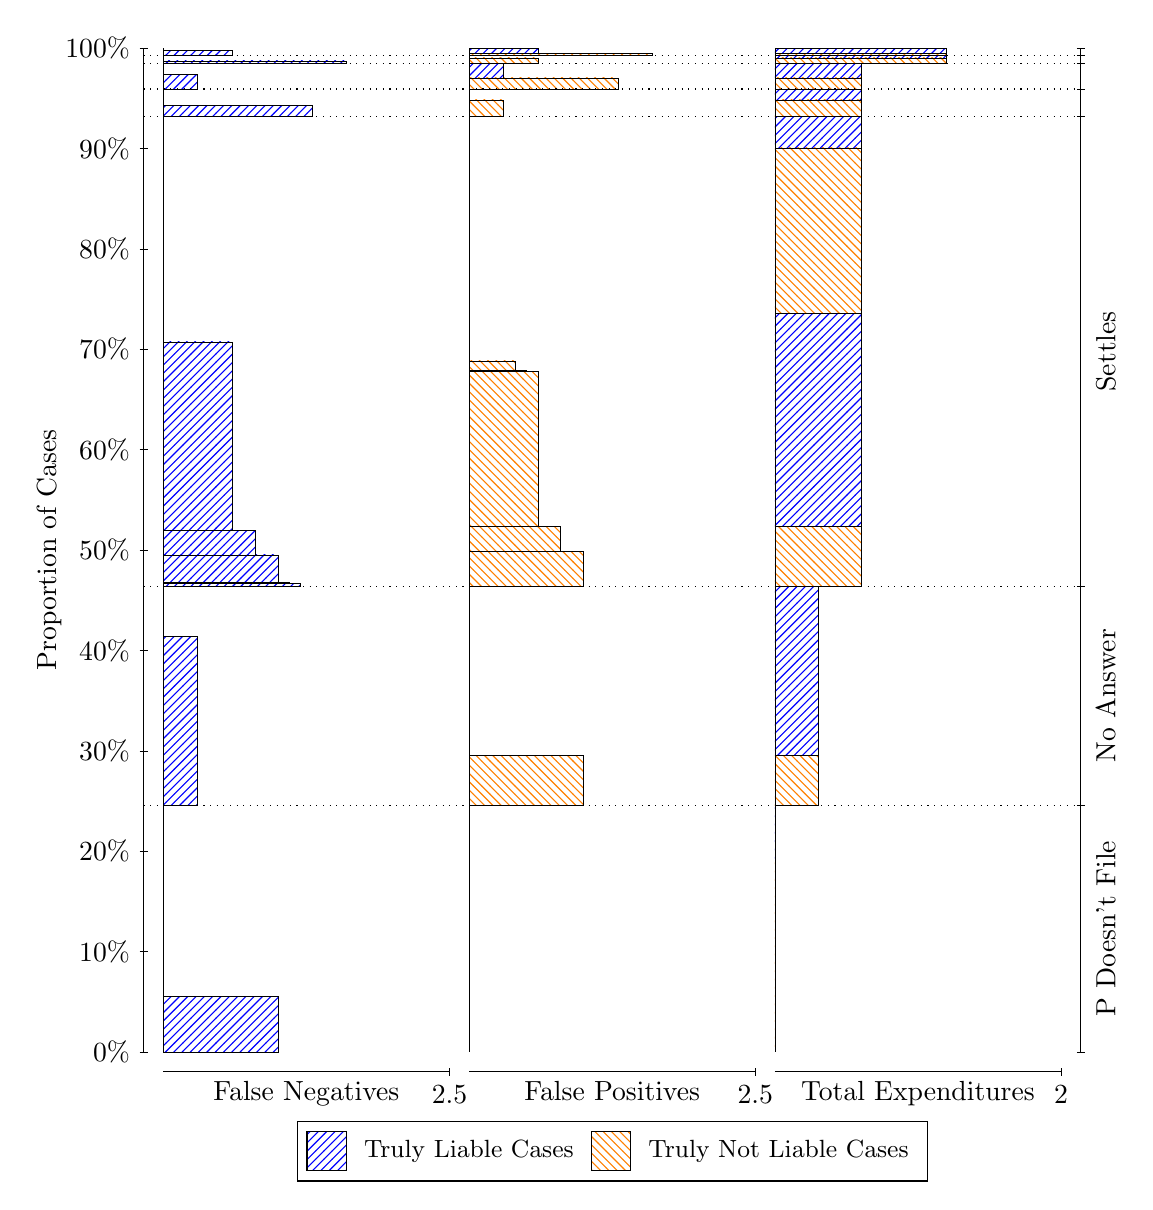
\begin{tikzpicture}
\draw[black, very thin] (1.5,1.75) -- (1.5,14.5);
\node[rotate=90, text=black, anchor=center] at (0.3, 8.125) {Proportion of Cases};
\draw[black, very thin] (1.45,1.75) -- (1.55,1.75);
\node[text=black, anchor=east] at (1.45, 1.75) {0\%};
\draw[black, very thin] (1.45,3.025) -- (1.55,3.025);
\node[text=black, anchor=east] at (1.45, 3.025) {10\%};
\draw[black, very thin] (1.45,4.3) -- (1.55,4.3);
\node[text=black, anchor=east] at (1.45, 4.3) {20\%};
\draw[black, very thin] (1.45,5.575) -- (1.55,5.575);
\node[text=black, anchor=east] at (1.45, 5.575) {30\%};
\draw[black, very thin] (1.45,6.85) -- (1.55,6.85);
\node[text=black, anchor=east] at (1.45, 6.85) {40\%};
\draw[black, very thin] (1.45,8.125) -- (1.55,8.125);
\node[text=black, anchor=east] at (1.45, 8.125) {50\%};
\draw[black, very thin] (1.45,9.4) -- (1.55,9.4);
\node[text=black, anchor=east] at (1.45, 9.4) {60\%};
\draw[black, very thin] (1.45,10.675) -- (1.55,10.675);
\node[text=black, anchor=east] at (1.45, 10.675) {70\%};
\draw[black, very thin] (1.45,11.95) -- (1.55,11.95);
\node[text=black, anchor=east] at (1.45, 11.95) {80\%};
\draw[black, very thin] (1.45,13.225) -- (1.55,13.225);
\node[text=black, anchor=east] at (1.45, 13.225) {90\%};
\draw[black, very thin] (1.45,14.5) -- (1.55,14.5);
\node[text=black, anchor=east] at (1.45, 14.5) {100\%};

\draw[black, very thin] (13.4,1.75) -- (13.4,14.5);
\draw[black, very thin] (13.35,1.75) -- (13.45,1.75);
\node[anchor=west] at (13.35, 1.75) {};
\draw[black, very thin] (13.35,4.882) -- (13.45,4.882);
\node[anchor=west] at (13.35, 4.882) {};
\draw[black, very thin] (13.35,7.6663) -- (13.45,7.6663);
\node[anchor=west] at (13.35, 7.6663) {};
\draw[black, very thin] (13.35,13.629) -- (13.45,13.629);
\node[anchor=west] at (13.35, 13.629) {};
\draw[black, very thin] (13.35,13.98) -- (13.45,13.98);
\node[anchor=west] at (13.35, 13.98) {};
\draw[black, very thin] (13.35,14.306) -- (13.45,14.306);
\node[anchor=west] at (13.35, 14.306) {};
\draw[black, very thin] (13.35,14.405) -- (13.45,14.405);
\node[anchor=west] at (13.35, 14.405) {};
\draw[black, very thin] (13.35,14.5) -- (13.45,14.5);
\node[anchor=west] at (13.35, 14.5) {};

\draw[black, very thin, pattern color=blue, pattern=north east lines] (1.75,1.75) rectangle (3.2033,2.4559);
\draw[black, very thin, pattern color=orange, pattern=north west lines] (1.75,2.4559) rectangle (1.75,4.882);
\draw[black, very thin, pattern color=blue, pattern=north east lines] (1.75,4.882) rectangle (2.186,7.0298);
\draw[black, very thin, pattern color=orange, pattern=north west lines] (1.75,7.0298) rectangle (1.75,7.6663);
\draw[black, very thin, pattern color=blue, pattern=north east lines] (1.75,7.6663) rectangle (3.494,7.7042);
\draw[black, very thin, pattern color=blue, pattern=north east lines] (1.75,7.7042) rectangle (3.3487,7.7099);
\draw[black, very thin, pattern color=blue, pattern=north east lines] (1.75,7.7099) rectangle (3.2033,8.0633);
\draw[black, very thin, pattern color=blue, pattern=north east lines] (1.75,8.0633) rectangle (2.9127,8.375);
\draw[black, very thin, pattern color=blue, pattern=north east lines] (1.75,8.375) rectangle (2.622,10.767);
\draw[black, very thin, pattern color=orange, pattern=north west lines] (1.75,10.767) rectangle (1.75,13.629);
\draw[black, very thin, pattern color=blue, pattern=north east lines] (1.75,13.629) rectangle (3.6393,13.769);
\draw[black, very thin, pattern color=orange, pattern=north west lines] (1.75,13.769) rectangle (1.75,13.98);
\draw[black, very thin, pattern color=blue, pattern=north east lines] (1.75,13.98) rectangle (2.186,14.166);
\draw[black, very thin, pattern color=orange, pattern=north west lines] (1.75,14.166) rectangle (1.75,14.306);
\draw[black, very thin, pattern color=blue, pattern=north east lines] (1.75,14.306) rectangle (4.0753,14.336);
\draw[black, very thin, pattern color=orange, pattern=north west lines] (1.75,14.336) rectangle (1.75,14.405);
\draw[black, very thin, pattern color=blue, pattern=north east lines] (1.75,14.405) rectangle (2.622,14.47);
\draw[black, very thin, pattern color=orange, pattern=north west lines] (1.75,14.47) rectangle (1.75,14.5);
\draw[black, very thin, pattern color=orange, pattern=north west lines] (5.6333,1.75) rectangle (5.6333,4.176);
\draw[black, very thin, pattern color=blue, pattern=north east lines] (5.6333,4.176) rectangle (5.6333,4.882);
\draw[black, very thin, pattern color=orange, pattern=north west lines] (5.6333,4.882) rectangle (7.0867,5.5184);
\draw[black, very thin, pattern color=blue, pattern=north east lines] (5.6333,5.5184) rectangle (5.6333,7.6663);
\draw[black, very thin, pattern color=orange, pattern=north west lines] (5.6333,7.6663) rectangle (7.0867,8.1076);
\draw[black, very thin, pattern color=orange, pattern=north west lines] (5.6333,8.1076) rectangle (6.796,8.425);
\draw[black, very thin, pattern color=orange, pattern=north west lines] (5.6333,8.425) rectangle (6.5053,10.39);
\draw[black, very thin, pattern color=orange, pattern=north west lines] (5.6333,10.39) rectangle (6.36,10.406);
\draw[black, very thin, pattern color=orange, pattern=north west lines] (5.6333,10.406) rectangle (6.2147,10.528);
\draw[black, very thin, pattern color=blue, pattern=north east lines] (5.6333,10.528) rectangle (5.6333,13.629);
\draw[black, very thin, pattern color=orange, pattern=north west lines] (5.6333,13.629) rectangle (6.0693,13.841);
\draw[black, very thin, pattern color=blue, pattern=north east lines] (5.6333,13.841) rectangle (5.6333,13.98);
\draw[black, very thin, pattern color=orange, pattern=north west lines] (5.6333,13.98) rectangle (7.5227,14.121);
\draw[black, very thin, pattern color=blue, pattern=north east lines] (5.6333,14.121) rectangle (6.0693,14.306);
\draw[black, very thin, pattern color=orange, pattern=north west lines] (5.6333,14.306) rectangle (6.5053,14.375);
\draw[black, very thin, pattern color=blue, pattern=north east lines] (5.6333,14.375) rectangle (5.6333,14.405);
\draw[black, very thin, pattern color=orange, pattern=north west lines] (5.6333,14.405) rectangle (7.9587,14.435);
\draw[black, very thin, pattern color=blue, pattern=north east lines] (5.6333,14.435) rectangle (6.5053,14.5);
\draw[black, very thin, pattern color=orange, pattern=north west lines] (9.5167,1.75) rectangle (9.5167,4.176);
\draw[black, very thin, pattern color=blue, pattern=north east lines] (9.5167,4.176) rectangle (9.5167,4.882);
\draw[black, very thin, pattern color=orange, pattern=north west lines] (9.5167,4.882) rectangle (10.062,5.5184);
\draw[black, very thin, pattern color=blue, pattern=north east lines] (9.5167,5.5184) rectangle (10.062,7.6663);
\draw[black, very thin, pattern color=orange, pattern=north west lines] (9.5167,7.6663) rectangle (10.607,8.425);
\draw[black, very thin, pattern color=blue, pattern=north east lines] (9.5167,8.425) rectangle (10.607,11.129);
\draw[black, very thin, pattern color=orange, pattern=north west lines] (9.5167,11.129) rectangle (10.607,13.232);
\draw[black, very thin, pattern color=blue, pattern=north east lines] (9.5167,13.232) rectangle (10.607,13.629);
\draw[black, very thin, pattern color=orange, pattern=north west lines] (9.5167,13.629) rectangle (10.607,13.841);
\draw[black, very thin, pattern color=blue, pattern=north east lines] (9.5167,13.841) rectangle (10.607,13.98);
\draw[black, very thin, pattern color=orange, pattern=north west lines] (9.5167,13.98) rectangle (10.607,14.121);
\draw[black, very thin, pattern color=blue, pattern=north east lines] (9.5167,14.121) rectangle (10.607,14.306);
\draw[black, very thin, pattern color=orange, pattern=north west lines] (9.5167,14.306) rectangle (11.697,14.375);
\draw[black, very thin, pattern color=blue, pattern=north east lines] (9.5167,14.375) rectangle (11.697,14.405);
\draw[black, very thin, pattern color=orange, pattern=north west lines] (9.5167,14.405) rectangle (11.697,14.435);
\draw[black, very thin, pattern color=blue, pattern=north east lines] (9.5167,14.435) rectangle (11.697,14.5);
\draw[black, dotted] (1.5,4.882) -- (13.4,4.882);
\draw[black, dotted] (1.5,7.6663) -- (13.4,7.6663);
\draw[black, dotted] (1.5,13.629) -- (13.4,13.629);
\draw[black, dotted] (1.5,13.98) -- (13.4,13.98);
\draw[black, dotted] (1.5,14.306) -- (13.4,14.306);
\draw[black, dotted] (1.5,14.405) -- (13.4,14.405);
\draw[black, very thin] (1.75,1.5) -- (5.3833,1.5);
\node[text=black, anchor=north] at (3.5667, 1.5) {False Negatives};
\draw[black, very thin] (5.3833,1.45) -- (5.3833,1.55);
\node[text=black, anchor=north] at (5.3833, 1.45) {2.5};

\draw[black, very thin] (5.6333,1.5) -- (9.2667,1.5);
\node[text=black, anchor=north] at (7.45, 1.5) {False Positives};
\draw[black, very thin] (9.2667,1.45) -- (9.2667,1.55);
\node[text=black, anchor=north] at (9.2667, 1.45) {2.5};

\draw[black, very thin] (9.5167,1.5) -- (13.15,1.5);
\node[text=black, anchor=north] at (11.333, 1.5) {Total Expenditures};
\draw[black, very thin] (13.15,1.45) -- (13.15,1.55);
\node[text=black, anchor=north] at (13.15, 1.45) {2};

\node[text=black, centered, rotate=90] at (13.72, 3.316) {P Doesn't File};
\node[text=black, centered, rotate=90] at (13.72, 6.2741) {No Answer};
\node[text=black, centered, rotate=90] at (13.72, 10.648) {Settles};





\draw (7.449999999999999,1.5) node[draw=none] (baseCoordinate) {};
\begin{scope}[align=center]
        \matrix[scale=0.5, draw=black, below=0.5cm of baseCoordinate, nodes={draw}, column sep=0.1cm]{
            \node[rectangle, draw, minimum width=0.5cm, minimum height=0.5cm, pattern color=blue, pattern=north east lines] {}; &
            \node[draw=none, font=\small, text=black] (B) {Truly Liable Cases}; &
            \node[rectangle, draw, minimum width=0.5cm, minimum height=0.5cm, pattern color=orange, pattern=north west lines] {}; &
            \node[draw=none, font=\small, text=black] (B) {Truly Not Liable Cases}; \\
            };
\end{scope}

\end{tikzpicture}
\end{document}